% -*- latex -*-
%%%%%%%%%%%%%%%%%%%%%%%%%%%%%%%%%%%%%%%%%%%%%%%%%%%%%%%%%%%%%%%%
%%%%%%%%%%%%%%%%%%%%%%%%%%%%%%%%%%%%%%%%%%%%%%%%%%%%%%%%%%%%%%%%
%%%%
%%%% This text file is part of the source of 
%%%% `Introduction to High-Performance Scientific Computing'
%%%% by Victor Eijkhout, copyright 2012/3/4/5/
%%%%
%%%% This book is distributed under a Creative Commons Attribution 3.0
%%%% Unported (CC BY 3.0) license and made possible by funding from
%%%% The Saylor Foundation \url{http://www.saylor.org}.
%%%%
%%%%
%%%%%%%%%%%%%%%%%%%%%%%%%%%%%%%%%%%%%%%%%%%%%%%%%%%%%%%%%%%%%%%%
%%%%%%%%%%%%%%%%%%%%%%%%%%%%%%%%%%%%%%%%%%%%%%%%%%%%%%%%%%%%%%%%

This section contains several simple codes that illustrate various
issues relating to the performance of a single CPU. The explanations
can be found in section~\ref{sec:performance-programming}.

\Level 1 {Preliminaries}

\Level 2 {Hardware event counting}
\label{sec:papi}

The codes in this chapter make calls to a library named PAPI for
`Performance Application Programming
Interface'~\cite{papi,papi-homepage}. This is a portable set of calls
to query the hardware counters that are built into most
processors. Since these counters are part of the processor hardware,
they can measure detailed events such as cache misses without this
measurement process disturbing the phenomenon it is supposed to
observe.

While using hardware counters is fairly straightforward, the question
of whether what they are reporting is what you actually meant to
measure is another matter altogether. For instance, the presence of
hardware prefetch streams (section~\ref{sec:prefetch}) implies that
data can be loaded into cache without this load being triggered by a
cache miss. Thus, the counters may report numbers that seem off, or
even impossible, under a naive interpretation.

\Level 2 {Test setup}

In the next sections you will see several codes that try to do 
precise timings on some phenomenon. This requires some care if you
want to be sure you are actuallying timing what you're interested in, and
not something else. 

First of all, of course you perform your experiment 
multiple times to get a good average timing. If the individual timings
are too far apart, you can decide to throw away outliers, or maybe
rethink your experiment: there may be a variable that you haven't accounted
for.

Let's assume that your timings are all within an acceptable spread;
next you have to compensate for cache effects stemming from the fact that
you are doing an experiment multiple times. If your problem sizes is small,
the first timing will bring all data in cache, and the second run
will find it there, leading to much faster runtimes. You can solve this 
problem by, in between any pair of timings, touching an array
that is larger than the cache size. This has the effect of flushing
all experiment data from the cache.

On the other hand, if you want to time something that happens on data
in cache, you want to be sure that your data is in cache, so you could
for instance write to the array, bringing it in cache, prior to your
experiment. This is sometimes referred to
as \indextermbus{cache}{warming}, and a cache that contains the
problem data is called a \indextermsub{hot}{cache}. Failure to warm
the cache leads to an results where the first run takes appreciably 
longer than the rest.

\Level 2 {Memory issues}
\label{sec:memalign}

For performance reasons it is often desirable to enforce
\indextermbus{cacheline}{boundary aligment} of data.
The easiest solution is to use \indextermsub{static}{allocation},
which puts the data on cacheline boundaries.

To put dynamically aligned data on cacheline boundaries, the
following code does the tric:
\begin{verbatim}
double *a;
a = malloc( /* some number of bytes */ +8 );
if ( (int)a % 8 != 0 ) { /* it is not 8-byte aligned */
  a += 1; /* advance address by 8 bytes, then */
  /* either: */
  a = ( (a>>3) <<3 );
  /* or: */
  a = 8 * ( ( (int)a )/8 );
}
\end{verbatim}
This code allocates a block of memory, and, if necessary, shifts it
right to have a starting address that is a multiple of~8.

However, a better solution is to use \indextermttdef{posix\_memalign}:
\begin{verbatim}
int posix_memalign(
  void **memptr, size_t alignment, size_t size);
\end{verbatim}
which allocates \n{size} bytes, aligned to a multiple of \n{alignment} bytes.
For example:
\begin{verbatim}
double x;
posix_memalign( (void**)&x,64,N*sizeof(double) );
\end{verbatim}
will allocate 64~doubles for~\n{x}, and align the array
to cacheline boundaries if there are 8 words per cacheline.

(If the \indextermbus{Intel}{compiler} complains about
\n{posix_memalign} being declared implicitly, add the \n{-std=gnu99}
flag to the compile line.

\Level 1 {Cache size}
\label{sec:cachesize-code}

This code demonstrates the fact that operations are more efficient if
data is found in L1 cache, than in L2, L3, or main memory. To make
sure we do not measure any unintended data movement, we perform one
iteration to bring data in the cache before we start the timers.

\begingroup\small
\verbatiminput{code/papi/size.c}
\endgroup

\Level 1 {Cachelines}
\label{sec:cacheline-code}

This code illustrates the need for small strides in vector code. The
main loop operates on a vector, progressing by a constant stride. As
the stride increases, runtime will increase, since the number of
cachelines transferred increases, and the bandwidth is the dominant
cost of the computation.

There are some subtleties to this code: in order to prevent accidental
reuse of data in cache, the computation is preceded by a loop that
accesses at least twice as much data as will fit in cache. As a
result, the array is guaranteed not to be in cache.

\begingroup\small
\verbatiminput{code/papi/line.c}
\endgroup

Note that figure~\ref{fig:cacheline} in
section~\ref{sec:coding-cacheline} only plots up to stride~8, while
the code computes to~16. In fact, at stride~12 the prefetch behaviour
of the Opteron changes, leading to peculiarities in the timing, as
shown in figure~\ref{fig:cacheline16}.
\begin{figure}[ht]
  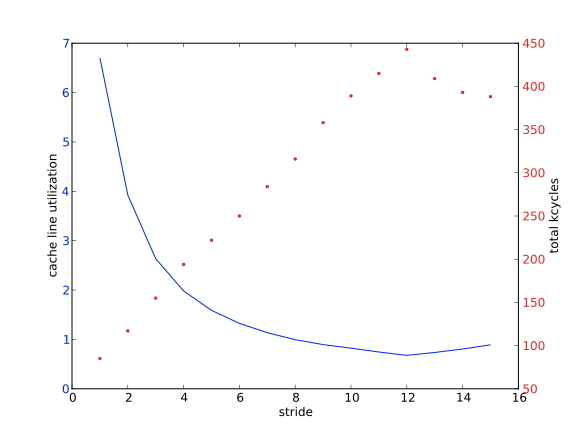
\includegraphics[scale=.5]{graphics/cacheline16}
  \caption{Run time in kcycles and L1 reuse as a function of stride}
  \label{fig:cacheline16}
\end{figure}

\Level 1 {Cache associativity}
\label{sec:assoc-code}

This code illustrates the effects of cache associativity;see sections
\ref{sec:associative} and~\ref{sec:assoc-coding} for a detailed
explanation. A~number of vectors (dependent on the inner loop
variable~\n{i}) is traversed simultaneously.  Their lengths are
chosen to induce cache conflicts. If the number of vectors is low
enough, cache associativity will resolve these conflicts; for higher
values of~\n{m} the runtime will quickly increase. By allocating the
vectors with a larger size, the cache conflicts go away.

\begingroup\small
\verbatiminput{code/papi/assoc.c}
\endgroup

\Level 1 {TLB}
\label{sec:tlb-code}

This code illustrates the behaviour of a \indexac{TLB}; see sections
\ref{sec:tlb} and~\ref{sec:coding-tlb} for a thorough
explanation. A~two-dimensional array is declared in column-major
ordering (Fortran style). This means that striding through the data by
varying the $i$~coordinate will have a high likelihood of TLB hits,
since all elements on a page are accessed consecutively. The number of
TLB entries accessed equals the number of elements divided by the page
size. Striding through the array by the $j$ coordinate will have each
next element hitting a new page, so TLB misses will ensue when the
number of columns is larger than the number of TLB entries.

\begingroup\small
\verbatiminput{code/papi/tlb.c}
\endgroup

\Level 1 {Unrepresentible numbers}
\label{sec:fraction-code}

Section~\ref{sec:arith-intro} mentioned that many fractions are not
representible in binary. This code illustrates that by dividing a
number first by~7, then multiplying it by~7 and dividing
by~49. Compile and execute this code, and see that an input of~$3.5$
gives equality, but $3.6$ doesn't.

\begingroup\small
\verbatiminput{code/snippets/fraction.c}
\endgroup
